\documentclass[11pt,a4paper]{article}
\usepackage[english]{babel}					% Use english
\usepackage[utf8]{inputenc}					% Caracteres UTF-8
\usepackage{graphicx}						% Imagenes
\usepackage[hidelinks]{hyperref}			% Poner enlaces sin marcarlos en rojo
\usepackage{fancyhdr}						% Modificar encabezados y pies de pagina
\usepackage{float}							% Insertar figuras
\usepackage[textwidth=390pt]{geometry}		% Anchura de la pagina
\usepackage[nottoc]{tocbibind}				% Referencias (no incluir num pagina indice en Indice)
\usepackage{enumitem}						% Permitir enumerate con distintos simbolos
\usepackage[T1]{fontenc}					% Usar textsc en sections
\usepackage{amsmath}						% Símbolos matemáticos
\usepackage{amsfonts}
\usepackage{subcaption}

% Comando para poner el nombre de la asignatura
\newcommand{\subject}{Numerical Linear Algebra}
\newcommand{\autor}{Vladislav Nikolov Vasilev}
\newcommand{\titulo}{Project 1}
\newcommand{\subtitulo}{Direct methods in optimization with constraints}
\newcommand{\masters}{Master in Fundamental Principles of Data Science}


% Configuracion de encabezados y pies de pagina
\pagestyle{fancy}
\lhead{\autor{}}
\rhead{\subject{}}
\lfoot{\masters}
\cfoot{}
\rfoot{\thepage}
\renewcommand{\headrulewidth}{0.4pt}		% Linea cabeza de pagina
\renewcommand{\footrulewidth}{0.4pt}		% Linea pie de pagina

\begin{document}
\pagenumbering{gobble}

% Title page
\begin{titlepage}
  \begin{minipage}{\textwidth}
    \centering
    
\includegraphics[scale=0.25]{img/ub-logo}\\[2cm]
    
    \textsc{\Large \subject\\[0.5cm]}
    \textsc{\uppercase\expandafter{\masters}}\\[1.5cm]
    
    \noindent\rule[-1ex]{\textwidth}{1pt}\\[1.5ex]
    \textsc{{\Huge \titulo\\[0.5ex]}}
    \textsc{{\Large \subtitulo\\}}
    \noindent\rule[-1ex]{\textwidth}{2pt}\\[3.5ex]
  \end{minipage}
  
  \vspace{2cm}
  
  \begin{minipage}{\textwidth}
    \centering
    
    
\includegraphics[scale=0.4]{img/ub-ds-logo}
    \vspace{2cm}
    
    \textbf{Author}\\ {\autor{}}\\[2.5ex]
    \textsc{Faculty of Mathematics and Computer Science}\\
    \vspace{1em}
    \textsc{Academic year 2021-2022}
  \end{minipage}
\end{titlepage}

\pagenumbering{arabic}
\tableofcontents
\thispagestyle{empty}				% No usar estilo en la pagina de indice

\newpage

\setlength{\parskip}{1em}

\section{Introduction}

The main goal of this project is to study the basic numerical linear algebra
behind optimization problems. In this case, we are going to consider a convex
optimization problem which has equality and inequality constraints. The goal
is to find a value of $x \in \mathbb{R}^n$ that solves the following
problem:

\begin{equation}
  \label{eq:minimization-problem}
  \begin{aligned}
    \text{minimize } &f(x) = \frac{1}{2}x^TGx + g^Tx \\
    \text{subject to } &A^Tx = b, \quad C^Tx \geq d
  \end{aligned}
\end{equation}

This constrained minimization problem can be solved using Lagrange multipliers.
In order to do so, we have to transform the inequality constraints into equality
constraints. Therefore, we introduce the slack variable $s = C^Tx - d \in \mathbb{R}^m, s \geq 0$.
The Lagrangian is given by the following expression:

\begin{equation}
  \label{eq:lagrangian}
  L(x, \gamma, \lambda, s) = \frac{1}{2}x^TGx + g^Tx - \gamma^T(A^Tx - b) - \lambda^T(C^Tx - d - s)
\end{equation}

The previous expression can be rewritten as:

\begin{equation}
  \label{eq:system}
  \begin{aligned}
    Gx + g - A\gamma - C\lambda &= 0\\
    b - A^T x &= 0 \\
    s + d - C^Tx &= 0 \\
    s_i \lambda_i &= 0, \quad i = 1, \dots, m
  \end{aligned}  
\end{equation}

To solve this problem, we are going to use the Newton's method. Additionally, each step
of the method is going to have two correction substeps that that will help us stay in the feasible
region of the problem.

\noindent \textbf{T1:} In order to solve this problem, let us define $z = (x, \gamma, \lambda, s)$ and
$F: \mathbb{R}^N \rightarrow \mathbb{R}^N$, where $N = n + p + 2m$. The function $F$ can be defined
as follows:

\[
  F(z) = F(x, \gamma, \lambda, s) = (Gx + g - A\gamma - C\lambda, b - A^T x, s + d - C^Tx, s_i \lambda_i)
\]

Our goal is to solve $F(z) = 0$ using Newton's method. This involves computing a Newton step
$\delta_z$ so that for a given point $z_k$ we have that $z_{k+1} = z_k + \delta_z, \forall k \in \mathbb{N}$.
Knowing that $F(z_{k+1}) = F(z_k) + J_F\delta_z$, we can see that this is equivalent to
solving the system $J_F\delta_z = -F(z_k)$, where $J_F$ is the Jacobian matrix.
This matrix is defined as follows:

\[
  J_F =
  \begin{pmatrix}
    \frac{\partial F_1}{\partial x} & \frac{\partial F_1}{\partial \gamma} &
    \frac{\partial F_1}{\partial \lambda} & \frac{\partial F_1}{\partial s} \\
    \frac{\partial F_2}{\partial x} & \frac{\partial F_2}{\partial \gamma} &
    \frac{\partial F_2}{\partial \lambda} & \frac{\partial F_2}{\partial s} \\
    \frac{\partial F_3}{\partial x} & \frac{\partial F_3}{\partial \gamma} &
    \frac{\partial F_3}{\partial \lambda} & \frac{\partial F_3}{\partial s} \\
    \frac{\partial F_4}{\partial x} & \frac{\partial F_4}{\partial \gamma} &
    \frac{\partial F_4}{\partial \lambda} & \frac{\partial F_4}{\partial s}
  \end{pmatrix}
  =
  \begin{pmatrix}
    G & -A & -C & 0 \\
    -A^T & 0 & 0 & 0 \\
    -C^T & 0 & 0 & I \\
    0 & 0 & S & \Lambda
  \end{pmatrix}
  :=
  M_{\text{KKT}}
\]

\noindent where $I$ is a $m \times m$ identity matrix and $S$ and $\Lambda$ are $m \times m$
diagonal matrices containing the values of $s$ and $\lambda$, respectively.

Thus, in order to obtain $\delta_z$ at each step, we have to solve a linear system of equations
defined by the matrix $M_{\text{KKT}}$ and the right hand vector $-F(z_k)$.


\section{Solving the KKT system without inequalities}

The first case that we are going to study is the KKT system without inequalities.
This allows us to represent the matrix $M_{\text{KKT}}$ as a $3 \times 3$ block
matrix:

\begin{equation}
  \label{eq:3x3-kkt}
  M_{\text{KKT}} =
  \begin{pmatrix}
    G & -C & 0 \\
    -C^T & 0 & I \\
    0 & S & \Lambda
  \end{pmatrix}
\end{equation}

There are some strategies that we can follow in order to solve the linear system of
equations. First, we will start by discussing a \textit{naive} approach, and later on we will present
some more advanced strategies that will allow us to solve the linear system faster.

\subsection{Naive approach}

The first approach that we are going to discuss is the one that we have called \textit{naive}. It
is named this way because it is the first one that one can think of and is the most direct one.
This method consists in solving the system using the \texttt{numpy.linalg.solve} function.
This function uses one of \texttt{LAPACK}'s \texttt{gesv} routines, which basically solves the system
by computing the LU factorization using GEPP under the hood.

\noindent \textbf{C1, C2, C3:} To solve this exercises, we have defined a function called
\texttt{lu\_solver} which can be found in the \texttt{kktsolvers/inequality.py} script.
It uses the provided \texttt{Newton\_method} function to compute the step-size correction
and one more function called \texttt{solve\_system} which computes $F(z_k)$.

As we already know, this method is quite slow, since it solves the system with $\frac{2}{3}n^3 + \mathcal{O}(n^2)$
flops. Moreover, it is used twice per iteration of the Newton's method, which means that
the factorization has to be computed two times. This implies that big sized problems will take
quite some time until they are solved. There are some improvements that can be made, like computing
the LU factorization just once and storing it. However, it might be a better idea to explore
other alternatives.

Fortunately, we can make some changes to $M_{\text{MKKT}}$ matrix that will allow us to
solve the problem faster.

\subsection{Other strategies}

In this section we are going to discuss two strategies that we can use to speed up
the Newton's method.

\subsubsection{$LDL^T$ factorization}

The first strategy that we are going to talk about is the $LDL^T$ factorization. Given a symmetric
matrix $A$, we can express this matrix as $A = LDL^T$, where $L$ is a unitriangular lower matrix and
$D$ is a diagonal matrix. This method is faster than the LU factorization, it takes up less space (we
only need to store one lower triangular and one diagonal matrix) and is more stable in general.

\noindent \textbf{T2.1:} We can factorize our $M_{\text{KKT}}$ matrix provided that it is symmetric. In order to obtain one, we
can perform some manipulations on it. From $\eqref{eq:3x3-kkt}$ we can obtain the following linear system:

\begin{equation}
  \begin{aligned}
    G\delta_x - C\delta_{\lambda} &= -r_L \\
    -C^T\delta_x + I\delta_s &= -r_C \\
    S\delta_{\lambda} + \Lambda \delta s &= -r_s
  \end{aligned}
\end{equation}

Now, if we isolate $\delta_s$ from the last equation, we get:

\[
  \delta_s = \Lambda^{-1}(-r_s - S\delta_{\lambda})
\]

Substituting in the second row we get:

\begin{equation*}
  \begin{aligned}
    -C^T \delta_x + \Lambda^{-1}(-r_s - S\delta_{\lambda}) = -r_C \\
    -C^T \delta_x - \Lambda^{-1}S\delta_{\lambda} = -r_C + \Lambda^{-1}r_s
  \end{aligned}
\end{equation*}

This has the following matrix form:

\begin{equation}
  \begin{pmatrix}
    G & -C \\
    -C^T & -\Lambda^{-1}S
  \end{pmatrix}
  \begin{pmatrix}
    \delta_x \\
    \delta_{\lambda} \\
  \end{pmatrix}
  =
  -
 \begin{pmatrix}
   r_L \\
   r_C - \Lambda^{-1}r_s
 \end{pmatrix}
\end{equation}

Since $G$ is a symmetric positive definite matrix, $C$ appears both in its normal
forms and transposed, and the matrix product $-\Lambda^{-1}S$ is a diagonal (which
is symmetric by definition), we can clearly see that this version of the $M_{\text{KKT}}$
is also symmetric. Thus, the $LDL^T$ factorization can be applied to it.

\noindent \textbf{C4.1:} In the \texttt{kktsolvers/inequality.py} script you can find the
implementation of this exercise. The function is called \texttt{ldlt\_solver}. It computes
the $LDL^T$ factorization of the $2 \times 2$ $M_{\text{KKT}}$ block matrix and then solves an
upper triangular equation system using the \texttt{scipy.linalg.solve\_triangular} function,
which is way faster than solving a whole system like we were doing before. Then, it divides
the resulting vector by the diagonal matrix $D$, which has been implemented as an element-wise
division between the result vector and the diagonal vector. Finally, it solves an upper triangular
system, using this time $L^T$. This time, the factorization is only computed once and is stored
so that it can be reused later, which allows us to save some time.

\subsubsection{Cholesky factorization}

The second strategy that we want to discuss is the Cholesky factorization. Given a symmetric
positive definite matrix $A$, instead of computing its factorization as $A = LU$, we can compute
it as $A = GG^T$, where $G$ is a lower triangular matrix whose diagonal is positive. Recalling
the $LDL^T$ factorization, we had a lower unitriangular matrix $L$ and a diagonal matrix $D$.
Since $A$ is SPD, its diagonal entries are positive. Thus, we can define
$D = \text{diag}(\sqrt{d_1}, \dots, \sqrt{d_n})^2$, and from here we can
derive that $G = L \times \text{diag}(\sqrt{d_1}, \dots, \sqrt{d_n})$.

The Cholesky factorization performs better than the LU since it takes half the time to
be computed, takes less space in memory (only one lower triangular matrix has to be stored)
and is more stable in general, since it can be computed without pivoting, which allows
us to get better solutions.

\noindent \textbf{T2.2:} In order to apply the Cholesky factorization to our matrix, we have to
perform some transformations so that it becomes symmetric and positive definite. Once again, we
can obtain the following linear system from the expression $\eqref{eq:3x3-kkt}$:

\begin{equation*}
  \begin{gathered}
    G\delta_x - C\delta_{\lambda} = -r_L \\
    -C^T\delta_x + I\delta_s = -r_C \\
    S\delta_{\lambda} + \Lambda \delta s = -r_s
  \end{gathered}
\end{equation*}

Now, if we isolate $\delta_s$ in the second row, we get the following expression:

\[
  \delta_s = -r_C + C^T \delta_x
\]

Substituting $\delta_s$ in the third row we get:

\begin{equation*}
  \begin{gathered}
    S\delta_{\lambda} + \Lambda(-r_C + C^T \delta_x) = -r_s \\
    S\delta_{\lambda} - \Lambda r_C + \Lambda C^T \delta_x = -r_s \\
    S\delta_{\lambda} = -r_s + \Lambda r_C - \Lambda C^T \delta_x \\
    S\delta_{\lambda} = S^{-1}(-r_s + \Lambda r_C) - S^{-1}\Lambda C^T \delta_x
  \end{gathered}
\end{equation*}

Substituting $\delta_{\lambda}$ into the first row we get:

\begin{equation*}
  \begin{gathered}
    G\delta_x - C(S^{-1}(-r_s + \Lambda r_C) - S^{-1}\Lambda C^T \delta_x) = -r_L \\
    G\delta_x - CS^{-1}(-r_s + \Lambda r_C) + CS^{-1}\Lambda C^T \delta_x = -r_L \\
    G\delta_x + CS^{-1}\Lambda C^T \delta_x = -r_L + CS^{-1}(-r_s + \Lambda r_C) \\
    (G + CS^{-1}\Lambda C^T) \delta_x = -r_L + CS^{-1}(-r_s + \Lambda r_C)
  \end{gathered}
\end{equation*}

Let us define $\hat{G} = G + CS^{-1}\Lambda C^T$ and $\hat{r} = -CS^{-1}(-r_s + \Lambda r_C)$.
Substituting in the previous expression we obtain the following system:

\[
  \hat{G} \delta_x = -r_L - \hat{r}
\]

We can apply the Cholesky factorization to the matrix $\hat{G}$ if it is SPD. We know that the matrix
$G$ is SPD. If the product $CS^{-1}\Lambda C^T$ is also SPD, then we would have that $\hat{G}$
is also SPD and it can be factorized using this method.

\noindent \textbf{C4.2:} The \texttt{cholesky\_solver} function (found in the same file
as the previous two) implements the Cholesky factorization and solves the system. To compute the
factorization, we have used the \texttt{scipy.linalg.cholesky} function. The biggest
difference regarding the previous approaches is that here we don't use the $M_{\text{KKT}}$ matrix.
Instead, we compute $\hat{G}$ and then compute its Cholesky factorization and replace its value
(since its only used to compute the factorization). This allows us to save some extra memory because
we don't have to save both the factorization matrices and the $M_{\text{KKT}}$ matrix at
the same time.

\subsection{Experimentation}

Now that we have a general idea of the different approaches that we are going to use to solve
this particular problem, let us perform some experimentation on them to see how they behave.

We are going to generate matrices and vectors of different sizes according to the provided instructions.
The sizes that we are going to use, which corresponds to the value of $n$, are going to be 10, 25, 50,
100, 200, 500 and 1000. This way we will be able to see how each method performs when the size of the
problem increases. We are also going to set $r = 7$ as the random seed, so that the executions can be
easily reproducible.

We want to get some metrics for each method to see how well it performs, such as:

\begin{itemize}
  \item Execution time.
  \item Number of iterations until it converges.
  \item Squared error to the real solution, given by $\| -g - x \|_2$.
  \item Condition number for each iteration. The matrices that we are going to use are the following
  ones: $3 \times 3$ $M_\text{KKT}$ block matrix for the naive approach (LU factorization),
  $2 \times 2$ $M_\text{KKT}$ block matrix for $LDL^T$ factorization and $\hat{G}$ matrix for Cholesky factorization.
  The selected norm is the $\| \cdot \|_\infty $ norm because we had some trouble computing the condition number
  with the $\| \cdot \|_2$ norm.
\end{itemize}

Let us now comment the results that we have obtained. For every problem size, all methods need exactly
the same number of iterations to converge. The number of iterations varies between 16-18 depending on the
size of the model. The error for all of them is 0, so they arrive at the expected solution once the
Newton's method finishes.

In the figure \ref{fig:execution-time} we can observe the execution time of each model. For small problems,
the different methods behave more or less in the same way. However, once the problem size starts increasing,
we can clearly see that the LU factorization is the slowest one of them all. The  $LDL^T$ factorization
comes in second place and is actually quite fast, needing approximately one fifth of the time of the LU method
for the largest problem. Finally, we can see that the method that uses the Cholesky factorization is the
fastest one for bigger problems, needing less than one fifth of the time of the LU factorization and approximately
less than half the time that the $LDL^T$ needs.

\begin{figure}[H]
  \centering
  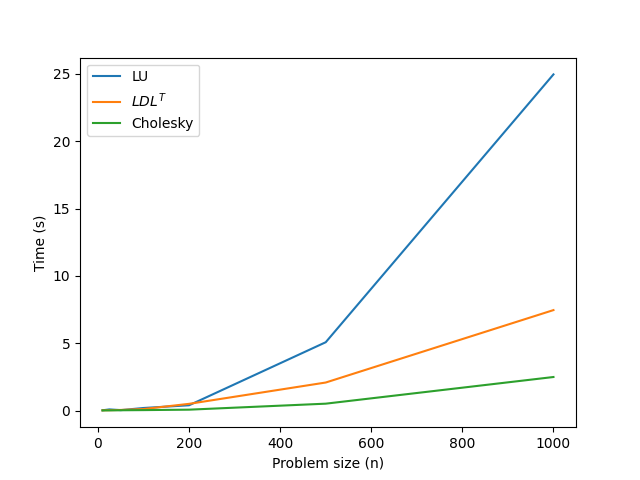
\includegraphics[scale=0.6]{img/inequality_times}
  \caption{Execution time of each method for different problem sizes.}
  \label{fig:execution-time}
\end{figure}

\begin{figure}[H]
  \centering
  \begin{subfigure}[t]{0.5\textwidth}
    \centering
    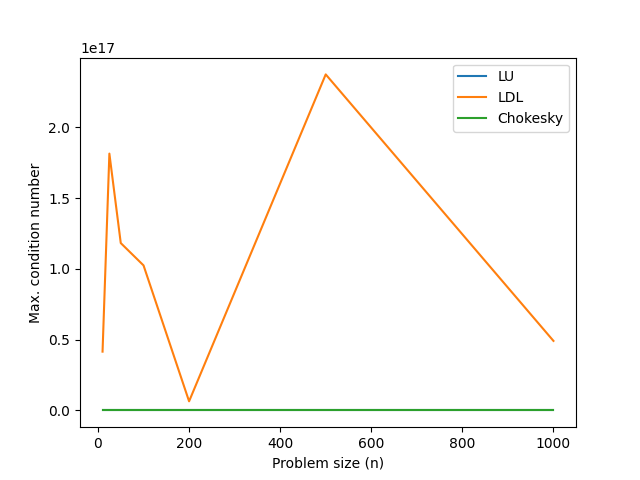
\includegraphics[scale=0.4]{img/max_cond_num_all}
    \caption{Maximum condition number for all methods.}
  \end{subfigure}%
  \begin{subfigure}[t]{0.5\textwidth}
    \centering
    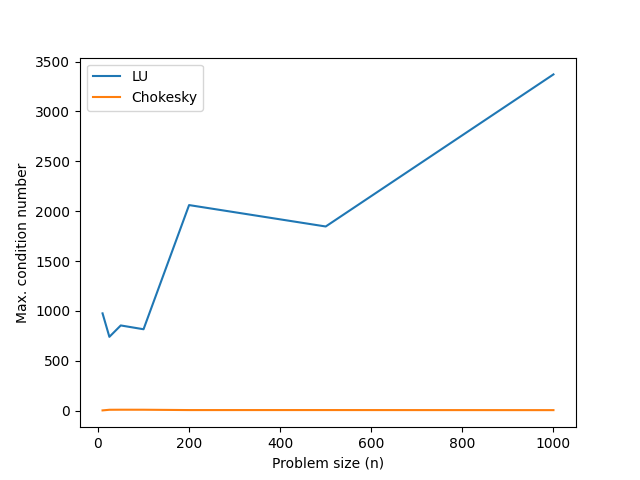
\includegraphics[scale=0.4]{img/max_cond_num_lu_cho}
    \caption{Maximum condition number for LU and Cholesky methods.}
  \end{subfigure}
  \caption{Evolution of the maximum condition number regarding the problem size.}
  \label{fig:max-cond-number}
\end{figure}

If we observe figure \ref{fig:max-cond-number}, we can see that the $LDL^T$ factorization
is the method with the highest maximum condition number for every problem size. The LU method
also has quite a large maximum condition number, but it is not comparable with the LU method.
The Cholesky method is the one with the smallest maximum condition number, which is no surprise at all
considering the fact that it is the most stable method among the three that we have studied.

\begin{figure}[H]
  \centering
  \begin{subfigure}[t]{0.5\textwidth}
    \centering
    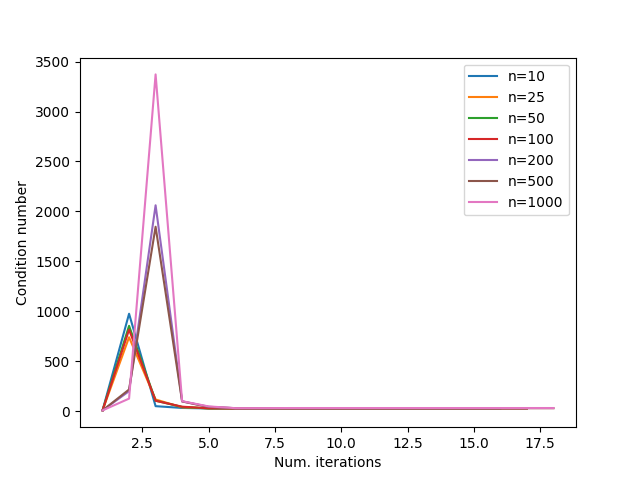
\includegraphics[scale=0.45]{img/cond_num_iter_lu}
    \caption{LU factorization.}
  \end{subfigure}%
  \begin{subfigure}[t]{0.5\textwidth}
    \centering
    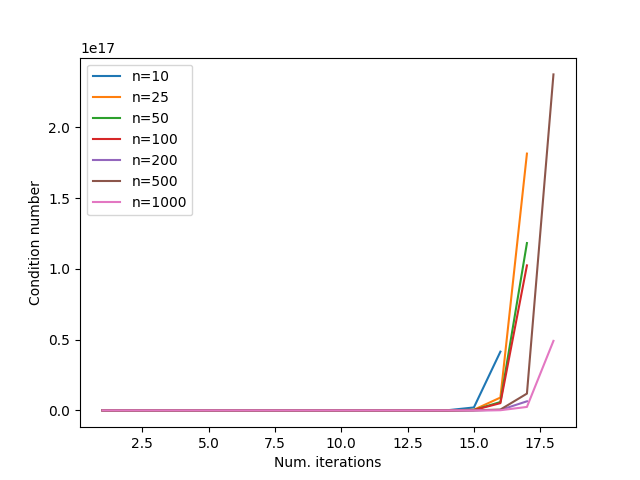
\includegraphics[scale=0.45]{img/cond_num_iter_ldl}
    \caption{$LDL^T$ factorization.}
  \end{subfigure}
  \vskip\baselineskip
  \begin{subfigure}[t]{0.5\textwidth}
    \centering
    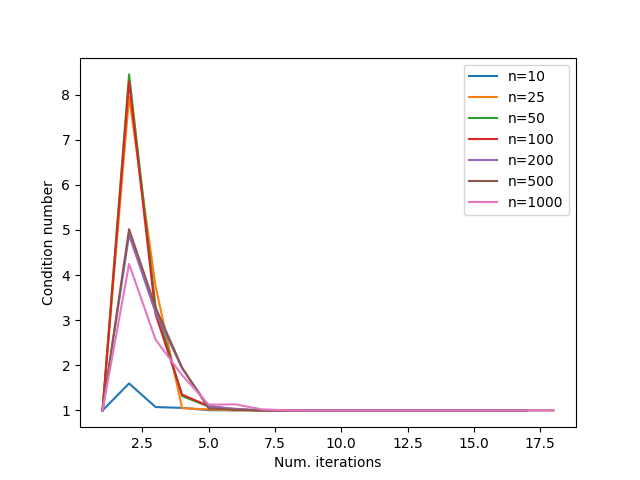
\includegraphics[scale=0.45]{img/cond_num_iter_cho}
    \caption{Cholesky factorization.}
  \end{subfigure}
  \caption{Evolution of the condition number of the three methods for all problem sizes.}
  \label{fig:ineq-cond-num-evolution}
\end{figure}

In the figure \ref{fig:ineq-cond-num-evolution} we can see more clearly how the condition number changes
as the different methods progress. For instance, for LU factorization we see how it spikes at the
beginning but then stabilizes. Something similar happens with the Cholesky factorization. However, its peak
is much smaller than the one from the LU factorization. The $LDL^T$ factorization behaves the other way around:
it seems stable at the beginning but, as we converge to the solution, it increases drastically. However,
since we are close to the stopping point, this doesn't have a lot of impact on the solution.
Recall also that previously we found out that the squared error was 0 for all solutions. Thus,
even if at some point the matrices may become ill or badly conditioned, they end up
stabilizing very quickly and converging to a good solution.

\section{Solving the general KKT system}

After getting acquainted with the KKT system without inequalities restrictions, it is
time that we try to solve the full system.

Just as we did before, we are going to try first a naive approach based on LU factorization, and
then we will try to modify the system so that we can apply another type of factorization to reduce
the execution time.

\subsection{Naive approach}

For this first approach, we have once again used the \texttt{numpy.linalg.solve} function
to solve the linear system. This time, however, we have a $4 \times 4$ block matrix, so
it is expected that it will take more time until the solution is found.

\noindent \textbf{C5:} The \texttt{kktsolvers/general.py} script includes a function called
\texttt{lu\_solver} that, as its name states, solves the general system using the LU
factorization. The difference with the previous one is that, in this case, we have
the $A$ matrix. Thus, the \texttt{solve\_system} function has been adapted so that when
$F(z_k)$ is computed, it also returns $r_A$. This way we can update the $\gamma$ variable.
Other than that, its inner workings are pretty much the same.

Just like before, this method suffers, in general, from poor performance. So, we are now
going to try another strategy that allows us to reduce the execution time. In this case,
we are going to try the $LDL^T$ factorization and see how it works.

\subsection{$LDL^T$ factorization}

\noindent \textbf{T3:} In order to apply the $LDL^T$ factorization, we have to transform the
$M_{\text{KKT}}$ matrix for the general KKT problem so that it is symmetric. Right now we have the
following linear system:

\begin{equation}
  \label{eq:kkt-general-system}
  \begin{pmatrix}
    G & -A & -C & 0 \\
    -A^T & 0 & 0 & 0 \\
    -C^T & 0 & 0 & I \\
    0 & 0 & S & \Lambda
  \end{pmatrix}
  \begin{pmatrix}
    \delta_x \\
    \delta_\gamma \\
    \delta_\lambda \\
    \delta_s
  \end{pmatrix}
  =
  -
  \begin{pmatrix}
    r_L \\
    r_A \\
    r_C \\
    r_s
  \end{pmatrix}
\end{equation}

We can represent the previous system as follows:

\begin{equation*}
  \begin{aligned}
    G\delta_x - A\delta_\gamma - C\delta_\lambda &= -r_L \\
    -A^T\delta_x &= -r_A \\
    -C^T\delta_x + I\delta_s &= -r_C \\
    S\delta_\lambda + \Lambda\delta_s &= -r_s
  \end{aligned}
\end{equation*}

If we isolate $\delta_s$ from the fourth row of the system, we obtain the following
expression:

\[
  \delta_s = -\Lambda^{-1}(r_s - S\delta_\lambda)
\]

We now substitute the previous result in the third row and get the following:

\begin{equation*}
  \begin{gathered}
    -C^T\delta_x - \Lambda^{-1}(r_s + S\delta_\lambda) = -r_C \\
    -C^T\delta_x - \Lambda^{-1}r_s - \Lambda^{-1}S\delta_\lambda = -r_C \\
    -C^T\delta_x - \Lambda^{-1}S\delta_\lambda = -r_c + \Lambda^{-1}r_s
  \end{gathered}
\end{equation*}

With these results, we can rewrite the $M_\text{KKT}$ system from expression
\eqref{eq:kkt-general-system} as

\begin{equation}
  \begin{pmatrix}
    G & -A & -C \\
    -A^T & 0 & 0 \\
    -C^T & 0 & -\Lambda^{-1}S
  \end{pmatrix}
  \begin{pmatrix}
    \delta_x \\
    \delta_\gamma \\
    \delta_\lambda
  \end{pmatrix}
  =
  -
  \begin{pmatrix}
    r_L \\
    r_A \\
    r_C - \Lambda^{-1}r_s
  \end{pmatrix}
\end{equation}

Like in the previous case, it is easy to see that the $3 \times 3$ $M_\text{KKT}$ block
matrix is symmetric. $G$ is a SPD matrix, and the $-\Lambda^{-1}S$ is a diagonal matrix,
which by definition is symmetric. In the matrix also appear the matrices $A$ and $C$ along
with their transposed versions, which means that they can be interchanged without any
problem. Thus, we see that our block matrix is symmetric, which implies that the $LDL^T$
factorization can be applied.

\noindent \textbf{C6:} The function \texttt{ldlt\_solver} from the same file as the previous
one is the responsible for performing the $LDL^T$ factorization and solving the problem.

Unfortunately, solving the system was not as straightforward as the last time. The culprit in this
case is the $D$ matrix, because the function \texttt{scipy.linalg.ldl} actually returns a block
diagonal matrix consisting of blocks of size at the most $2 \times 2$. In the previous case
we didn't have this problem because the $D$ matrix was always diagonal, without any blocks in it.
But here, there are some cases in which we can find elements adjacent to the main diagonal
that are non-zero, effectively showing that it is actually a block diagonal matrix.

There are some workarounds that we can perform to solve this issue. The first one is
to use the \texttt{scipy.linalg.lapack.dsysv}, a \texttt{LAPACK} routine that solves the system
directly performing the $LDL^T$ factorization under the hood. However, since using it feels like
defeating the purpose of this exercise, we have implemented two functions that helped us solve
this kind of systems.

The main responsible for solving the linear system is the \texttt{ldl\_block\_solver} function.
This function first permutes the $L$ matrix and the right hand vector using the permutation array
obtained from the $LDL^T$ factorization. This way, we bring the $L$ matrix into a lower triangular
one, and we permute the right hand vector accordingly. Also, we have to store the inverse permutation
so we can undo it later.

After that is done, the function solves 3 systems. The first one is a lower triangular system,
and it calls the \texttt{scipy.linalg.solve\_triangular} function. Then, it solves the
block diagonal system. There is no specific function for this, so we have created one that
is called \texttt{solve\_block\_diagonal}. The function iterates over the elements of the diagonal
and checks if the adjacent elements (the one on the right and below the current one) are zero or very
close to it (there might have been some perturbation in the computations, so we establish a threshold
to filter these values out). If the adjacent elements are below the threshold, then it divides the
corresponding element of the right hand vector by the current element of the diagonal. Otherwise, it
solves a $2 \times 2$ linear system using the \texttt{np.linalg.solve} function. For systems this small,
its performance is acceptable. Once this system is solved, the function solves an upper triangular
system. Finally, it applies the inverted permutation to the result vector so that the values come
back to their original positions.

\subsection{Experimentation}

Having defined the new approaches that we are going to use to solve the general system, we are going to
carry out now some experiments to see how well they actually perform.

We are given two problems: one of size $n = 100$, and the other one of size $n = 1000$. We are going to
try to solve them and see if we can get the solution or very close to it. Also, we would like to know
how much time it takes the two methods to converge and what are the condition numbers of the matrices.

For the first problem, both methods find exactly the same solution, which is $11590.7181$ approximately and
corresponds with the one that we are given. However, the LU method needs 22 iterations and $0.172$ seconds
approximately to reach it, whereas the $LDL^T$ method needs 23 iterations and $0.519$ seconds approximately.
The difference in iterations is not very significant, but the difference in time is. The reason behind this might
be that the implementation of the function that solves the block diagonal system is not optimized enough or
that it should be implemented in a lower level language.

If we study now the results obtained for the second problem, we see that both methods reach exactly the same
solution again, which is $1087511.5673$ approximately and corresponds with the given solution.
Unlike in the previous case, here the LU factorization needs 29 iterations and $58.85$ seconds approximately
to reach the solution, whereas the $LDL^T$ method requires 28 iterations and only $16.92$ seconds to reach
it. Once more, the difference in the number of iterations is not really significant. However, what is significant
is the time difference. In this case, the LU method is much slower than the $LDL^T$ factorization.

\begin{figure}[H]
  \centering
  \begin{subfigure}[t]{0.5\textwidth}
    \centering
    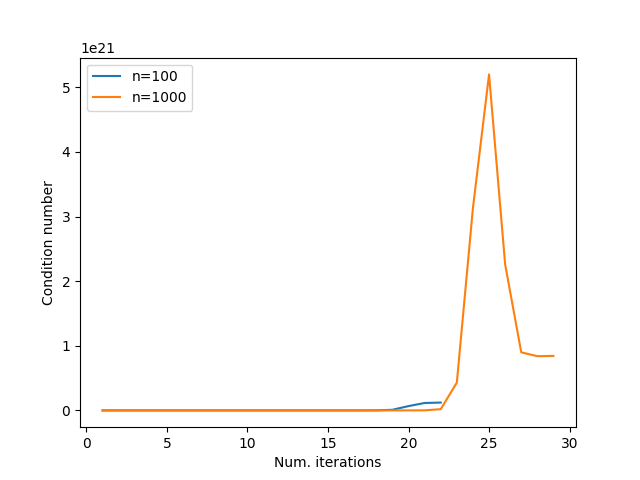
\includegraphics[scale=0.4]{img/equality_cond_iter_lu}
    \caption{LU factorization.}  
  \end{subfigure}%
  \begin{subfigure}[t]{0.5\textwidth}
    \centering
    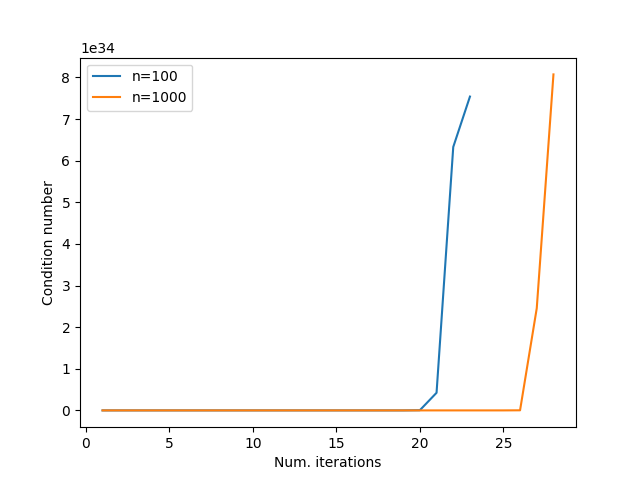
\includegraphics[scale=0.4]{img/equality_cond_iter_ldl}
    \caption{$LDL^T$ factorization.}  
  \end{subfigure}
  \caption{Evolution of the condition number for each method and each problem.}
  \label{fig:eq-cond-num}
\end{figure}

Now, in order to study the evolution of the condition number, we have computed the condition numbers
of the respective $M_\text{KKT}$ matrices of each method using again the $\| \cdot \|_\infty$ norm.

If we observe the figure \ref{fig:eq-cond-num}, we can see that that for the small problem, the condition number
of the LU method increases slightly at the end, but for the $LDL^T$ method it increases much drastically.
For the big problem, it increases a lot on both of them, but in the LU case it seems that it stabilizes after that.
Notice however that the values that are reached are very big (more than $10^20$), which would cause the matrix to be
ill-conditioned. But, since these changes occur usually at the end, they don't seem to affect the result at all since
the method is really close the solution.


\end{document}

